\chapter{The elsewhere allophones of the front lax vowels}
\label{ch:elsewhere_shift}

This chapter presents a description of the elsewhere allophones of the front lax vowels in Cowlitz County. Recall that these allophones of \trap, \dress, and \kit, are those that occur before obstruents (except /\textipa{g}/) and are most directly related to the Elsewhere Shift. \S\ref{BAT}--\ref{BIT} discuss the \bat, \bet, and \bit vowels, respectively, primarily based on visualizations of the model outputs for each vowel. In \S\ref{sec:preobstruent_discussion}, I summarize the findings and conclude the chapter with a brief discussion of the implications of these results. A more in-depth discussion of these findings, particularly as they relate to speakers' relationship with the Pacific Northwest and the mills, is presented in Chapter \ref{ch:discussion}.

% ---------------------------------------------------------------------------------
% ------------------------------    BAT    ----------------------------------------
% ---------------------------------------------------------------------------------

\section{\bat}
\label{BAT}

In this dataset, there were 5,702 tokens of \bat coming from 706 unique words. The most frequent of these words were \textit{back}, \textit{actually}, \textit{dad}, \textit{last}, \textit{bad}, \textit{castle}\footnote{Most tokens of \textit{castle} were in reference to the Cowlitz County city, Castle Rock.}, \textit{ash}, \textit{class}, \textit{half}, and \textit{happened}. The average number of tokens per speaker was 105\footnote{Speakers ranged from 48 to 204 tokens with a standard deviation of 37.1: 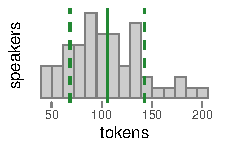
\includegraphics[width = 1.5in]{Figures/BAT/BAT_tiny.pdf}} and the average number of tokens per generation per sex was about 713. In this dataset, \bat varies considerably across ages and sexes and the patterns that are found in this sample reflect similar patterns described in other areas in the West.

\begin{figure*}[tb!]
	\centering
	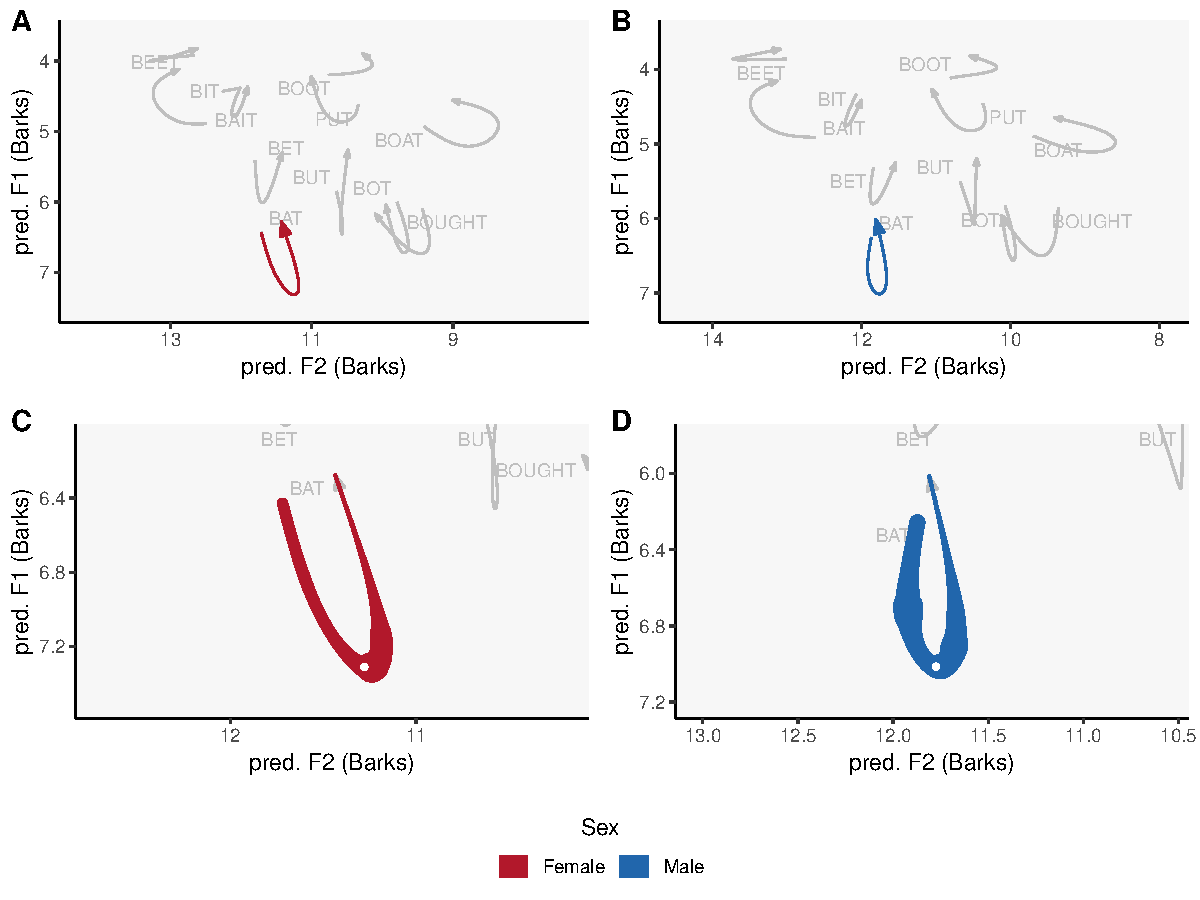
\includegraphics[width = 6.5in]{Figures/BAT/BAT_four_panel_plot_summarized.pdf}
	\caption[Predicted formant measurements for \bat by sex.]{Predicted formant measurements for \bat by sex with women on the left and men on the right. Predicted values are averaged across all generations.}
	\label{fig:BAT_four_panel_summarized}
\end{figure*}

Figure \ref{fig:BAT_four_panel_summarized} shows the effect that sex had on the \bat vowel in a four-panel plot.\footnote{For details on how to interpret this and subsequent plots, see \S\ref{sec:visualizing_gamms}} It is immediately clear that this vowel is not monophthongal but that there is some vowel-inherent spectral change. Specifically, the vowel gets lower during the first half of its duration before raising again during the second half. As seen in panels A and B, there is a fair amount of movement in \bat; the trajectory length was 2.002 Barks.\footnote{This is calculated by extracting predicted values for \bat at 501 time points and getting the sum of the Euclidean distances in the Bark F1-F2 space from each point to the next consecutive point. Basically, I apply the methods described by \citet{fox_jacewicz_2009}, only except taking the sum of 4 segments, I take the sum of 500 segments simply because I have the ability to extract that many predicted values from the GAMMs.} In fact, the trajectory length of \bat was the longest out of any allophone of any of the front lax vowels in this sample. However, at no point does \bat overlap with any other vowel, so \bat is contained in its own portion of the vowel space. There appears to be a clear target for this vowel for both F1 and F2 that is approximately at the halfway point of its duration. By ``target'' I mean that the visual shape of this trajectory achieves its lowest point at approximately the midpoint of its duration, suggesting that when these speakers pronounce this vowel, they do so by attempting to hit this point in the vowel space. There is no immediately obvious difference between the sexes in Figure \ref{fig:BAT_four_panel_summarized}, suggesting that the way this vowel is realized is approximately the same for both men and women.

\begin{figure*}[tb!]
	\centering
	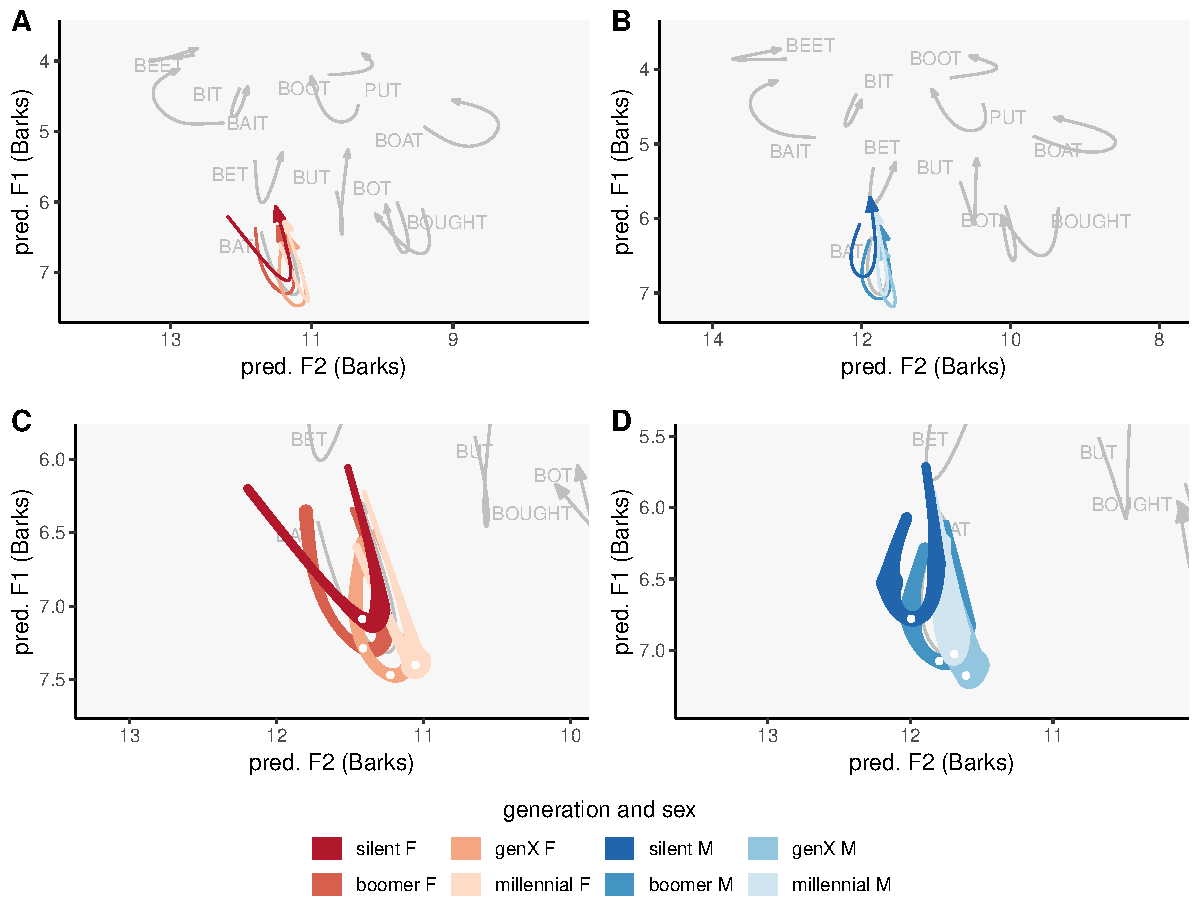
\includegraphics[width = 6.5in]{Figures/BAT/BAT_four_panel_plot.pdf}
	\caption[Predicted formant measurements for \bat by sex and generation.]{Predicted formant measurements for \bat by sex and generation. Women are on the left and men on the right. Darker shades represent older generations.}
	\label{fig:BAT_four_panel}
\end{figure*}

When the data is split up by the four generations in this sample and by sex, the differences between the sexes become more defined. Figure \ref{fig:BAT_four_panel} shows the predicted trajectories for \bat for each combination of generation and sex from the GAMM. Beginning with the women, we see that the target of \bat, which happens to occur near the midpoint of the vowel gradually lowers and then retracts. Difference smooths (Appendix \ref{appendix:difference_smooths}, Figure \ref{fig:bat_diff_smooths_gen}, Panels A--B, M--N, U--V) suggest that the change between successive generations of women was relatively small, but when comparing nonconsecutive generations the difference reaches statistical significance (\ref{fig:bat_diff_smooths_gen}, E--F, I--J, Q--R). For instance, compared to the Silent generation, Boomer women had no significant change in the height of \bat (\ref{fig:bat_diff_smooths_gen}A), and compared to the Boomers, neither did the Gen X women (\ref{fig:bat_diff_smooths_gen}M); but when compared to the Silent women, Gen X women had a significantly higher F1 (corresponding to a lower vowel) along the majority of its trajectory (\ref{fig:bat_diff_smooths_gen}E). Retraction of \bat occurred primarily in the first half of the vowel's trajectory and also in the later three generations, with each generation shifting a small portion of the beginning half to a more retracted portion of the vowel space. In summary, we see that the changes in the women's realizations of \bat include lowering and retraction, primarily in the first half of the trajectory.

Turning to the right panels in Figure \ref{fig:BAT_four_panel}, we can begin to analyze the men's realizations. Some of the patterns are shared with the women's realizations of \bat. For example, the Gen X men had a significantly lower realization of \bat than the Silent men along the entire course of its trajectory. However, difference smooths suggest that there are further changes that were not found in the women's data. For one, this pattern of lowering \bat was statistically significant between the oldest two generations, but only in the second half of the trajectory (\ref{fig:bat_diff_smooths_gen}C). There is also a pattern of retraction, though it is only large enough to reach statistical significance when comparing the Silent Generation to the two younger groups and is centered around the 25\% point in the duration of the vowel (\ref{fig:bat_diff_smooths_gen}H,L). So for the men, we find that the bulk of the changes occurred first in last half of \bat's trajectory where the younger generations used lowered offglides and then in the first half of the trajectory where younger generations used a fronter nucleus. It is noteworthy that these changes were not centered around the midpoint of the vowel, but it is indeed the trajectories of the vowel that are undergoing change.
%TODO: Dr. Renwick wants me to explain more about the last sentence in the previous paragraph.

Figure \ref{fig:BAT_four_panel} therefore suggests a pattern of gradual lowering and retraction, primarily in the first half of the vowel's trajectory, over the course of the four generations in this sample. This pattern is noticeably different from what was found in California, where the primary direction of change is in F2 \citep{donofrio_etal_2019}. Here, the differences between successive generations were generally small and were only noticeably when comparing speakers to their grandparents' or grandchildren's generation. It appears then that the lowering and retraction of \bat is active and has been steadily advancing for at least four generations in Cowlitz County.

\begin{figure*}[p]
	\centering
	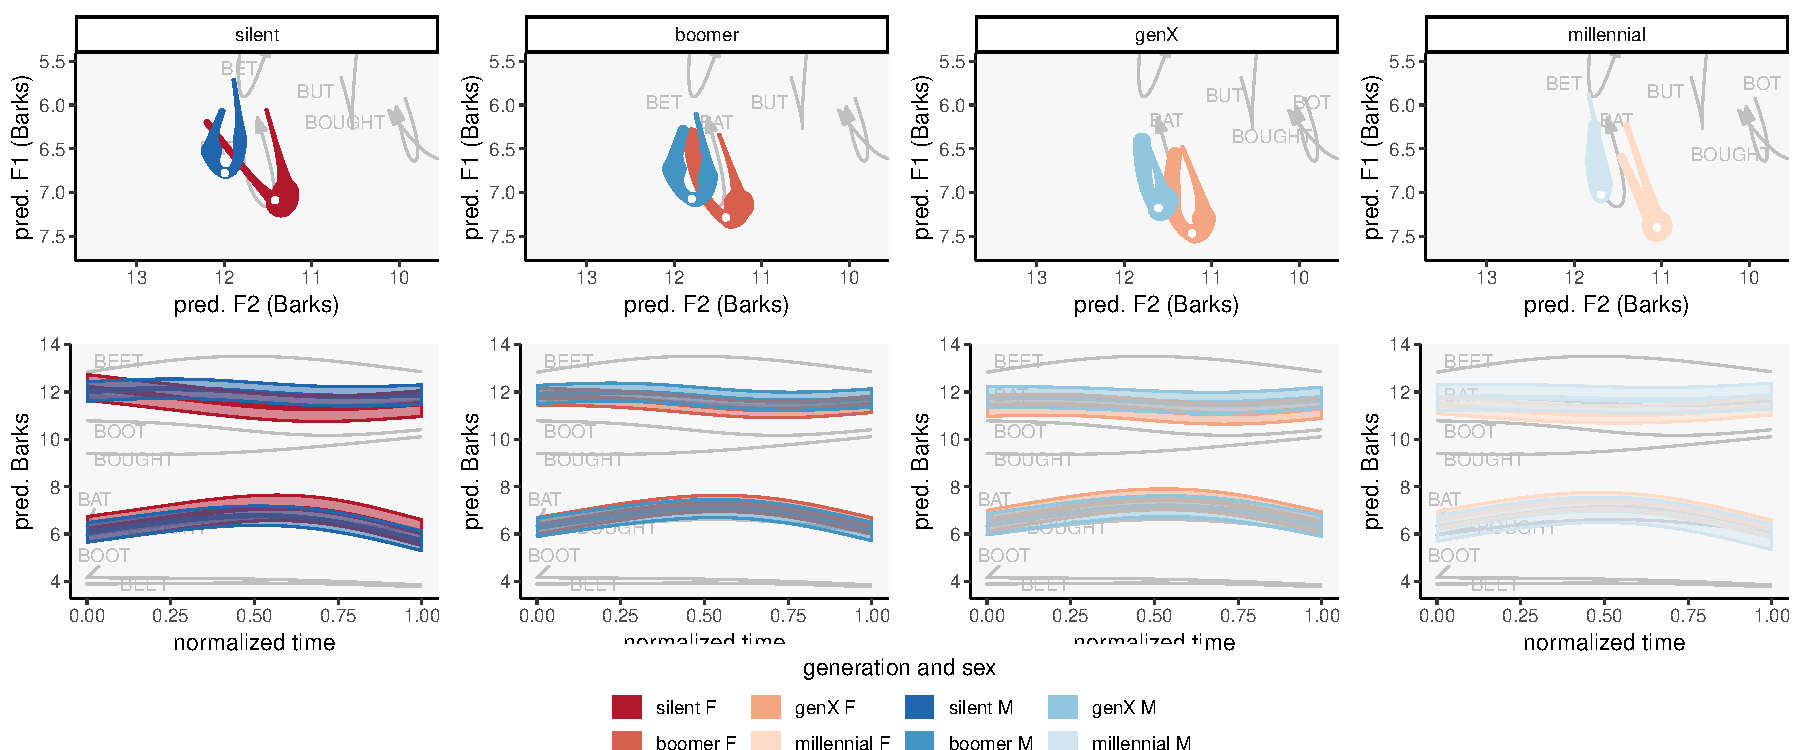
\includegraphics[angle = 90, origin = c, height = \textwidth]{Figures/BAT/BAT_sex_panel_plot_wide.pdf}
	\caption[Predicted formant measurements for \bat by generation.]{Predicted formant measurements for \bat by generation.}
	\label{fig:BAT_sex_panel_plot_wide}
\end{figure*}

As an alternative view of the data, Figure \ref{fig:BAT_sex_panel_plot_wide} shows the same predicted trajectory data but split up by generation rather than by sex. Because the data are normalized, an apples-to-apples comparison can be made between the sexes within each generation. This visualization makes it apparent that there are differences between the sexes in all generations and that these differences are roughly consistent in apparent time: women use a more lowered and retracted variant of \bat than men in their generation. Difference smooths between these pairs of predicted trajectories (Appendix \ref{appendix:difference_smooths}, Figure \ref{fig:bat_diff_smooths_sex_gen}) suggest that women lead this change both in F1 and F2 for all four generations, reaching statistical significance in most pairs. In the Silent generation, the difference is significant during the last half of the F1 trajectory and in all but the first 20\% of F2 (\ref{fig:bat_diff_smooths_sex_gen}A,B). Among the Boomers, the difference is slightly smaller, and is only significant in F2 (\ref{fig:bat_diff_smooths_sex_gen}C,D). For Gen X, the difference again only reached statistical significance for F2 (\ref{fig:bat_diff_smooths_sex_gen}E,F) suggesting that perhaps the men caught up with the women at least in the height dimension. But for the Millennials, the women's trajectory is significant different from the men's for the entire duration of the vowel for both F1 and F2 (\ref{fig:bat_diff_smooths_sex_gen}G,H). A trend in these difference smooths is that the significance is primarily found in the latter portion of the vowel's trajectory, suggesting that what makes men's and women's realizations of \bat is the realization of the entire offglide.

Taking Figures \ref{fig:BAT_four_panel} and \ref{fig:BAT_sex_panel_plot_wide} together, we see a clear case of language change in apparent time, with women in the lead. The differences across generations, which were primarily in the first half of the trajectory, were relatively small and did not often reach statistical significance between consecutive generations, but they add up to show a modest amount of change over the 67 years of apparent time data in this sample. Women are consistently ahead of mean in this change as well, especially in the second half of the trajectory. Putting these descriptions together, we see a continuous and relatively constant rate of change, but the complex nature of this shift, with different parts of the trajectory changing at different rates, highlights the need for analyzing trajectories rather than midpoints alone.


% ---------------------------------------------------------------------------------
% ------------------------------    BET    ----------------------------------------
% ---------------------------------------------------------------------------------
\section{\bet}
\label{BET}

In this sample, there were 7,943 tokens of \bet coming from 771 unique words. The most frequent of these words were \textit{said}, \textit{yes}, \textit{everything}, \textit{never}, \textit{every}, \textit{ever}, \textit{everybody}, \textit{whatever}, \textit{guess}, and \textit{together}. Because the GAMM included a random intercept for word, it adjusts for the fact that many of these words have the vowel followed by /\textipa{v}/. Each speaker produced an average of 143 tokens of \bet\footnote{Speakers ranged from 56 to 404 tokens with a standard deviation of 59.9: 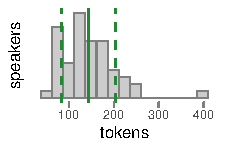
\includegraphics[width = 1.5in]{Figures/BET/BET_tiny.pdf}} resulting in approximately 997 per generation per sex.

\begin{figure*}[tb!]
	\centering
	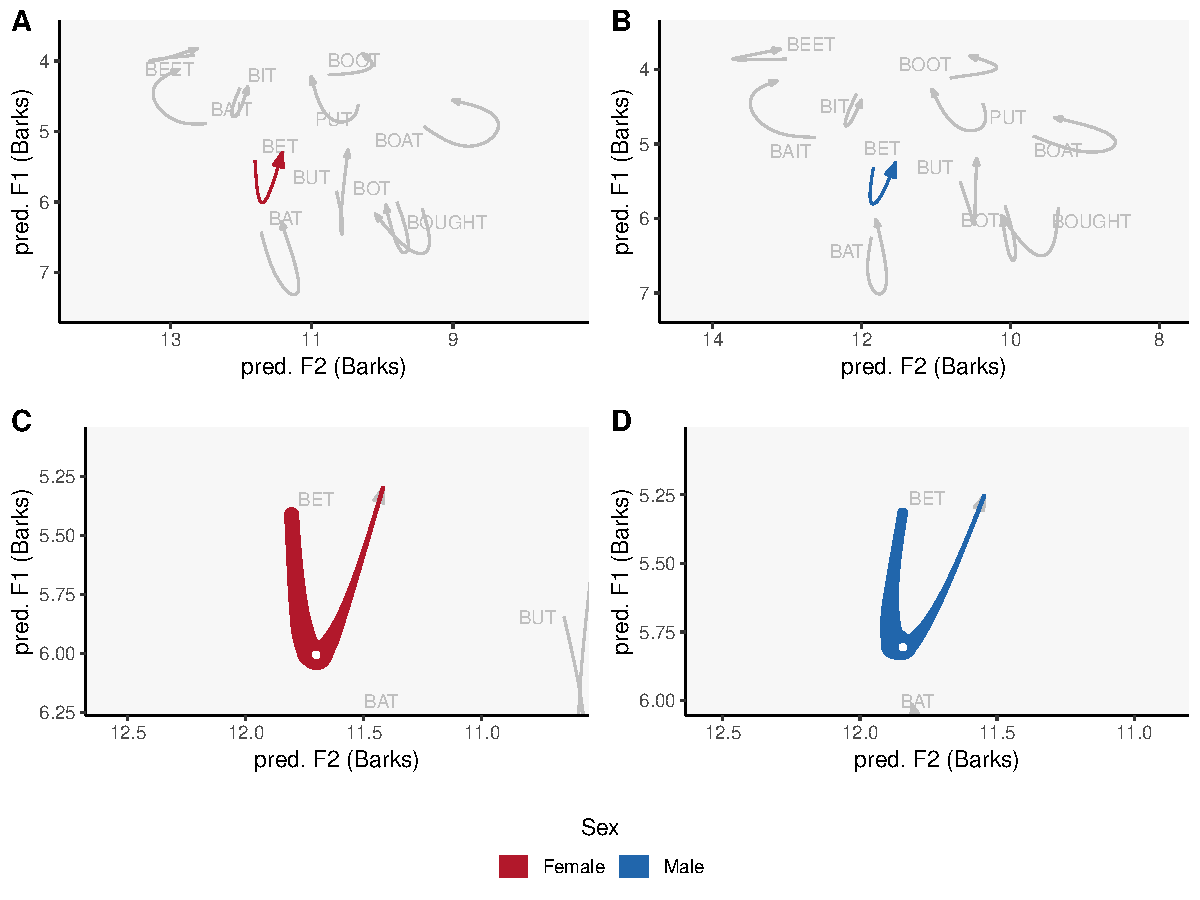
\includegraphics[width = 6.5in]{Figures/BET/BET_four_panel_plot_summarized.pdf}
	\caption[Predicted formant measurements for \bet by sex.]{Predicted formant measurements for \bet by sex with women on the left and men on the right. Predicted values are averaged across all generations.}
	\label{fig:BET_four_panel_summarized}
\end{figure*}

Figure \ref{fig:BET_four_panel_summarized} offers a first look at how \bet is realized in this sample. Regarding its relative position in the vowel space, \bet shares approximately the same F2 space as \bat but is equal in height with \strut and midway between the low back vowels and \goat. Compared to \bat, the shape of the trajectory of \bet is similar with an approximately U-shaped curve that starts fronter, reaches a clear target near the midpoint, and then ends more centralized. However, compared to \bat, panels A and B of Figure \ref{fig:BET_four_panel_summarized} show that the overall amount of movement that \bet undergoes is relatively small. In fact, while the predicted trajectory length of \bat was 2.002 Barks, \bet was only 1.264 Barks. Clearly \bet is more monophthongal than \bat in this sample. Comparing panels C and D, there are no obvious differences between the sexes when all generations are pooled together.

\begin{figure*}[tb!]
	\centering
	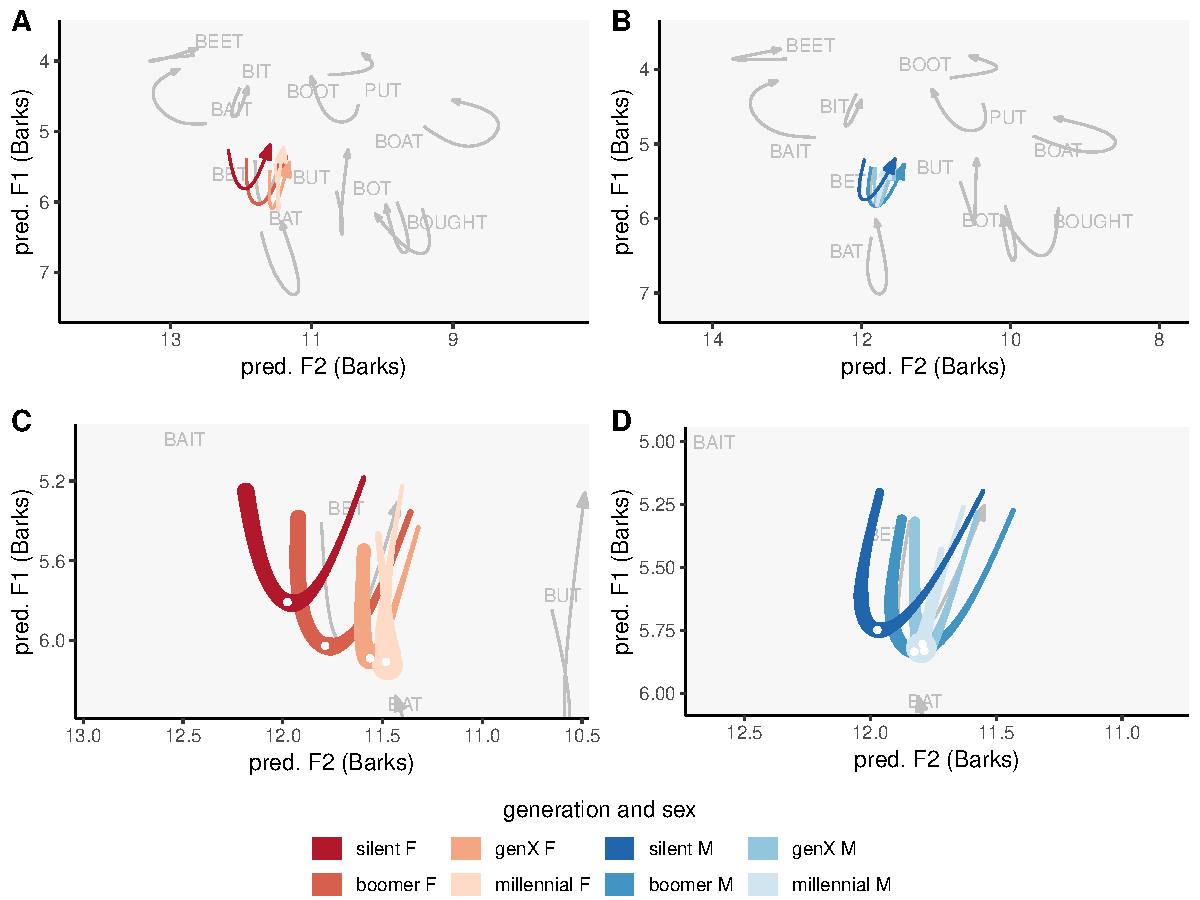
\includegraphics[width = 6.5in]{Figures/BET/BET_four_panel_plot.pdf}
	\caption[Predicted formant measurements for \bet by sex and generation.]{Predicted formant measurements for \bet by sex and generation. Women are on the left and men on the right. Darker shades represent older generations.}
	\label{fig:BET_four_panel}
\end{figure*}

Splitting the data by generation, as in Figure \ref{fig:BET_four_panel}, offers a more nuanced view at how \bet changes in apparent time. Beginning with the women on the left, panel C shows that \bet simultaneously lowers, retracts, and changes shape in apparent time. Like \bat, the change in the height of \bet is relatively small from one generation to the next (Appendix \ref{appendix:difference_smooths}, Figure \ref{fig:bet_diff_smooths_gen}A--B, M, U--V), but when skipping generations, difference smooths suggest that the lowering is statistically significant (\ref{fig:bet_diff_smooths_gen}E--F,I--J,R), but (again) only in the first half of the trajectory. The direction of change was greater along the F2 dimension and the first half of the trajectory was backed more than the offset. The largest jump in \bet retraction was between the Boomers and Gen X and did reach statistical significance, at least in the first half of the vowel's duration (\ref{fig:bet_diff_smooths_gen}N). Difference smooths suggest that the younger two generations had a significantly more retracted \bet than the Silent Generation for essentially the entire duration of the vowel (\ref{fig:bet_diff_smooths_gen}F,J); this is supported in panel C of Figure \ref{fig:BET_four_panel} where the onset of the Millennial women's \bet had a lower F2 than even the offset of that of the Silent women. The result of the onset shifting more than the offset is a change in trajectory shape in apparent time: the older generations have a more U-shaped curve where F2 gradually lowers over the course of the vowel's duration while the younger generations' \bet is ``pointier,'' culminating in Millennials' realizations with hardly any change in F2. While the entire vowel is lowering and retracting, it is doing so at an uneven rate and it appears that the onset has ``caught up'' to the offset. Speculatively, if this trend continues, future generations of Washington women may reverse the shape of \bet entirely, such that it starts as a central vowel and glides towards the front.

In stark contrast to the women's intriguing pattern, the men show relatively little change in \bet in apparent time. Superficially, panel D shows that the men exhibit a similar pattern of lowering, retraction, and reduction in the range of F2 that the vowel crosses through, but the amount of change from one generation to the next is small. In fact, difference smooths show no statistical significance in either F1 or F2 between any generation of men, except for a small portion near the onset that was significantly more retracted for the Millennials and Gen X than the Silent men, but this may not be found in other samples (\ref{fig:bet_diff_smooths_gen}H,L). In other words, \bet is relatively stable in this sample of Cowlitz County men and does not show change in apparent time.

\begin{figure*}[p]
	\centering
	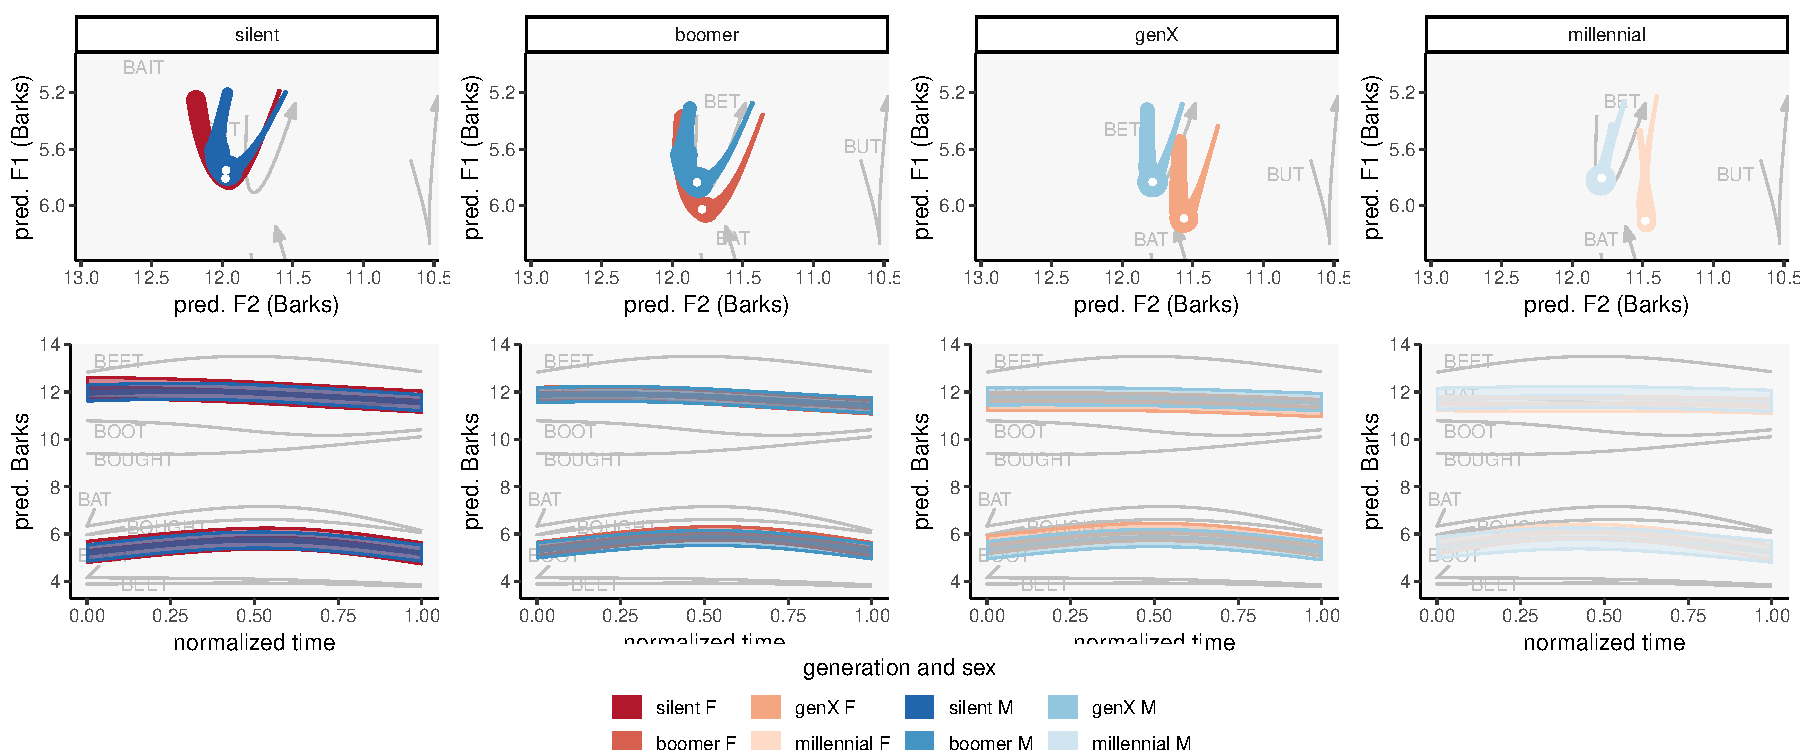
\includegraphics[angle = 90, origin = c, height = \textwidth]{Figures/BET/BET_sex_panel_plot_wide.pdf}
	\caption[Predicted formant measurements for \bet by generation.]{Predicted formant measurements for \bet by generation.}
	\label{fig:BET_sex_panel_plot_wide}
\end{figure*}

The question that remains then is how the women compare to the men in their relative positioning. Is it the case that the women are shifting away from the men or did the men start with a more centralized vowel and the women are shifting towards them? Figure \ref{fig:BET_sex_panel_plot_wide} provides evidence for the former. The leftmost panel of Figure \ref{fig:BET_sex_panel_plot_wide} plots the women and men in the Silent Generation and shows that they have very similar realizations of \bet, both in position and shape of the curve; difference smooths suggest no difference between the sexes. We can therefore conclude that there the oldest generation of speakers in this sample realized \bet the same way. However, Figure \ref{fig:BET_sex_panel_plot_wide} shows that as the speakers get younger, the sexes diverge. Among the Baby Boomers and Gen X, the difference is primarily in height, and difference smooths (\ref{fig:bet_diff_smooths_sex_gen}C,E) suggest a statistically significant difference in F1 just in the middle 15\% and third of the vowel, respectively. Between the Millennials, the difference in height expands to the middle 50\% of the vowel in F1 and the middle two-thirds for F2. In other words, difference smooths support what is visually apparent in Figure \ref{fig:BET_sex_panel_plot_wide}: men and women's realizations of \bet gradually separate with each successive generation. And the fact that the oldest generation started off with no difference between them suggests that there was no change at that time and that this sample captures the beginning of this vowel shift change in Cowlitz County.

In addition to their separation in apparent time, GAMMs provide an additional and intriguing insight when looking at \bet: the shape of the vowel trajectories was quite similar between the sexes across all generations. This is not a consequence of the model: recall that the GAMM fit each combination of sex and generation as independent factors, and though a human analyst knows that female Millennials have the same age range as male Millennials, the model was not ``aware'' of this fact. This makes it all the more surprising that each generation's vowel trajectories were similar in shape. So far in this analysis of \bet, I have suggested that language change is happening among the women but not the men. If only the midpoints were analyzed, this may be a reasonable conclusion. But while the men's realizations are relatively stable in the vowel space, their trajectories are in sync with the changes that the women are doing. These similarities across generations are a curious case of language change where men are keeping up with the women but only in one aspect of the shift. This also justifies the use of GAMMs because this kind of effect could not easily be detected if only one measurement were taken per vowel.

Summarizing the findings for \bet, this section has shown changes in apparent time that are conditioned by the sex of the speaker. Women are lowering, retracting, and changing the shape of \bet while men are simply changing its shape while remaining more or less in the same relative position in the vowel space. Specifically, the trajectory is changing such that the first half of the vowel is shifting faster than the second half, resulting in a change from a U-shape to a “bounce” in the F1-F2 space. Finally, the Baby Boomers initiated this shift since the differences between the sexes was negligible in the Silent generation.



% ---------------------------------------------------------------------------------
% ------------------------------    BIT    ----------------------------------------
% ---------------------------------------------------------------------------------

\section{\bit}
\label{BIT}


% I'll need to rerun the models after removing getting and different, maybe.
The final vowel to be analyzed in this chapter is \bit. In this sample, there were 8,231 tokens of \bit coming from 736 unique words. The most frequent of these words were \textit{different}, \textit{little}, \textit{kids}, \textit{pretty}, \textit{lived}, \textit{bit}, \textit{six}, \textit{live}, and \textit{river}. Each speaker produced an average of 152 tokens of \bit\footnote{Speakers ranged from 59 to 323 tokens with a standard deviation of 49.7: 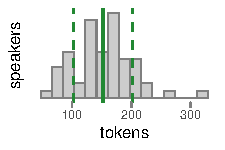
\includegraphics[width = 1.5in]{Figures/BIT/BIT_tiny.pdf}} meaning there were approximately 1029 per generation per sex.

\begin{figure*}[tb!]
	\centering
	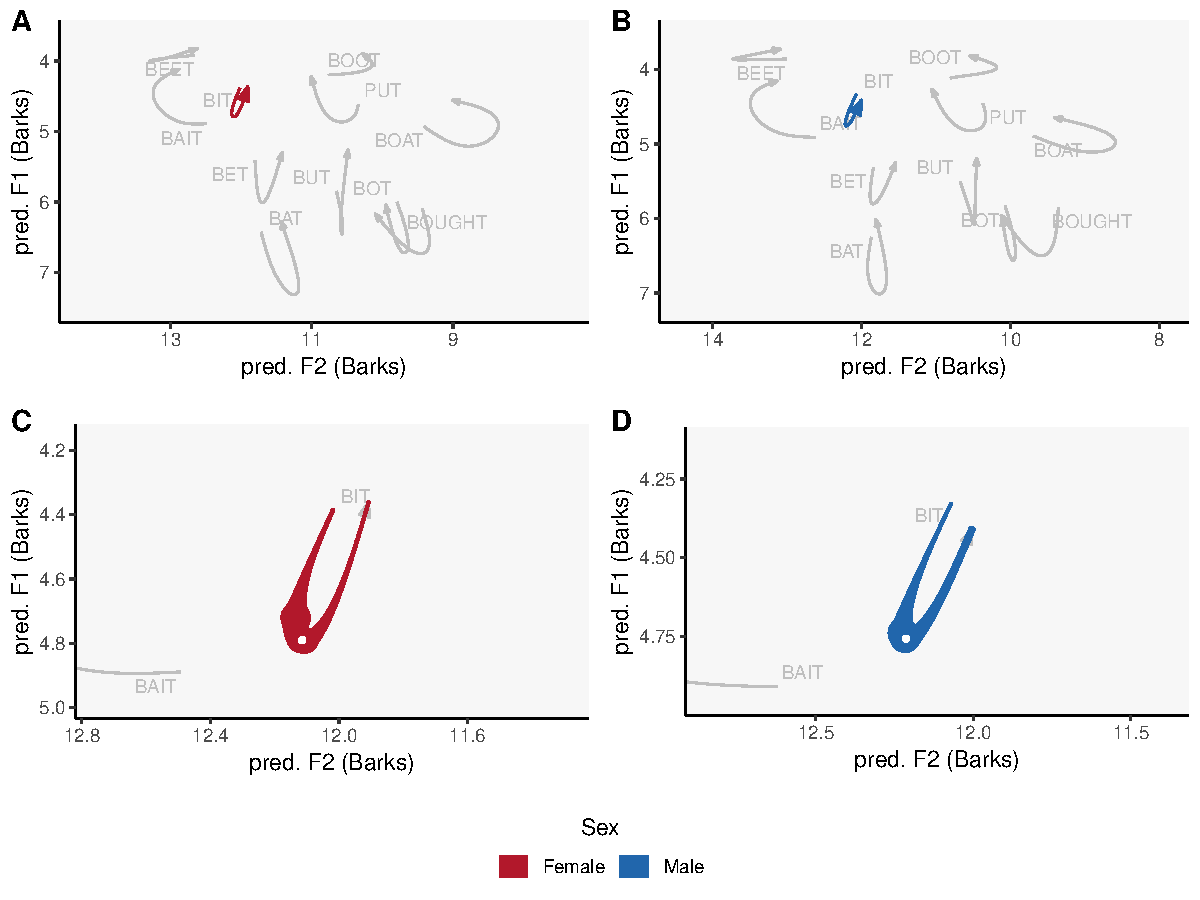
\includegraphics[width = 6.5in]{Figures/BIT/BIT_four_panel_plot_summarized.pdf}
	\caption[Predicted formant measurements for \bit by sex.]{Predicted formant measurements for \bit by sex with women on the left and men on the right. Predicted values are averaged across all generations.}
	\label{fig:BIT_four_panel_summarized}
\end{figure*}

Figure \ref{fig:BIT_four_panel_summarized} offers a preliminary analysis of \bit in this sample of Cowlitz County speakers. Its relative position compared to other vowels is that is about the same height as \face and \strut and slightly fronter than \bet and \bat. Like \bat and \bet, the \bit vowel takes on a U-shaped curve, starting higher and fronter, dipping towards a target near the midpoint, and ending at a point about as high as the onset but more centralized. However, it is the least dynamic vowel among the the front lax vowels with an average trajectory length of 0.903, which is slightly less than half the length of \bat. Like the other vowels, when the data is summarized for all speakers of the same sex as in Figure \ref{fig:BIT_four_panel_summarized}, there are no obvious differences between how men and women realize this vowel.

\begin{figure*}[tb!]
	\centering
	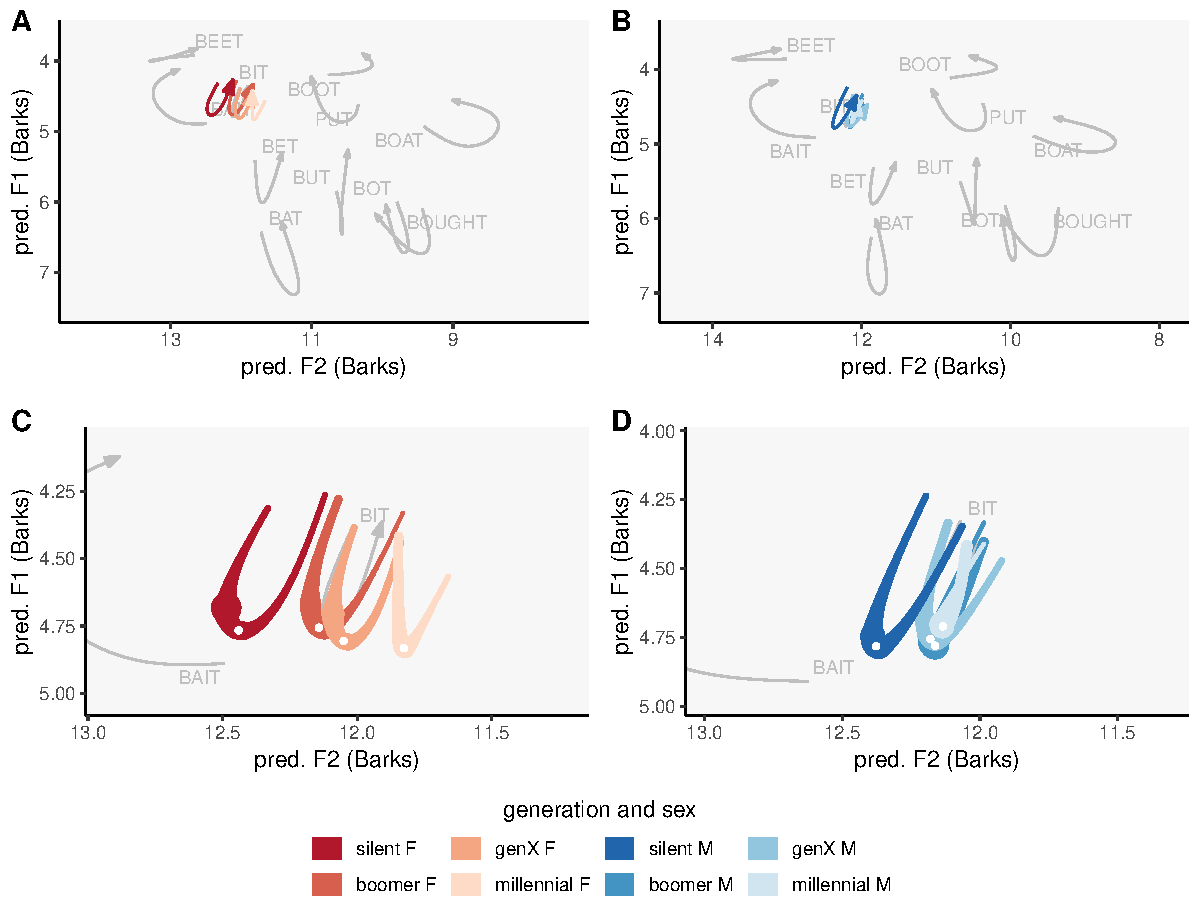
\includegraphics[width = 6.5in]{Figures/BIT/BIT_four_panel_plot.pdf}
	\caption[Predicted formant measurements for \bit by sex and generation.]{Predicted formant measurements for \bit by sex and generation. Women are on the left and men on the right. Darker shades represent older generations.}
	\label{fig:BIT_four_panel}
\end{figure*}

But, when the data is split up by sex and generation, then patterns in apparent time emerge. Panels A and C of Figure \ref{fig:BIT_four_panel} shows a pattern of \bit retraction in apparent time among the Cowlitz County women in this sample. The women in the Silent Generation use the most fronted variant of \bit, but with each generation the vowel becomes incrementally more retracted. The amount of change in the vowel space is relatively small, but difference smooths suggest that much of this retraction is statistically significant (\ref{fig:bit_diff_smooths_gen}B,F,J,R,V). From the Silent Generation to the Baby Boomers, the difference was significant along the entire trajectory of the vowel (\ref{fig:bit_diff_smooths_gen}B), which is supported by the lack of overlap between the two curves in Figure \ref{fig:BIT_four_panel}. Between the Baby Boomers and Gen X, the difference was not significant at all (\ref{fig:bit_diff_smooths_gen}N). But between Gen X and the Millennials, the first half of the trajectory was significantly more retracted (\ref{fig:bit_diff_smooths_gen}V). This on-again-off-again pattern of retraction may be indicative of the end of one shift and the beginning of a new phase of \bit retraction. Regarding vowel height, there was very little evidence of \bit lowering in this sample (\ref{fig:bit_diff_smooths_gen}A,E,I,M,Q,U)

Moving on to panels B and D of Figure \ref{fig:BIT_four_panel}, we see a pattern reminiscent of what was found with \bet: relatively little change. While the women are undergoing a gradual but robust process of \bit retraction, the men do not appear to be following suit. There is some degree of retraction between the oldest two generations of men, and the difference smooths suggest that the shift in the first half of the trajectory was statistically significant (\ref{fig:bit_diff_smooths_gen}D). But otherwise, \bit is remarkably stable among Cowlitz County men, at least in the vowel's position in the vowel space.

\begin{figure*}[p]
	\centering
	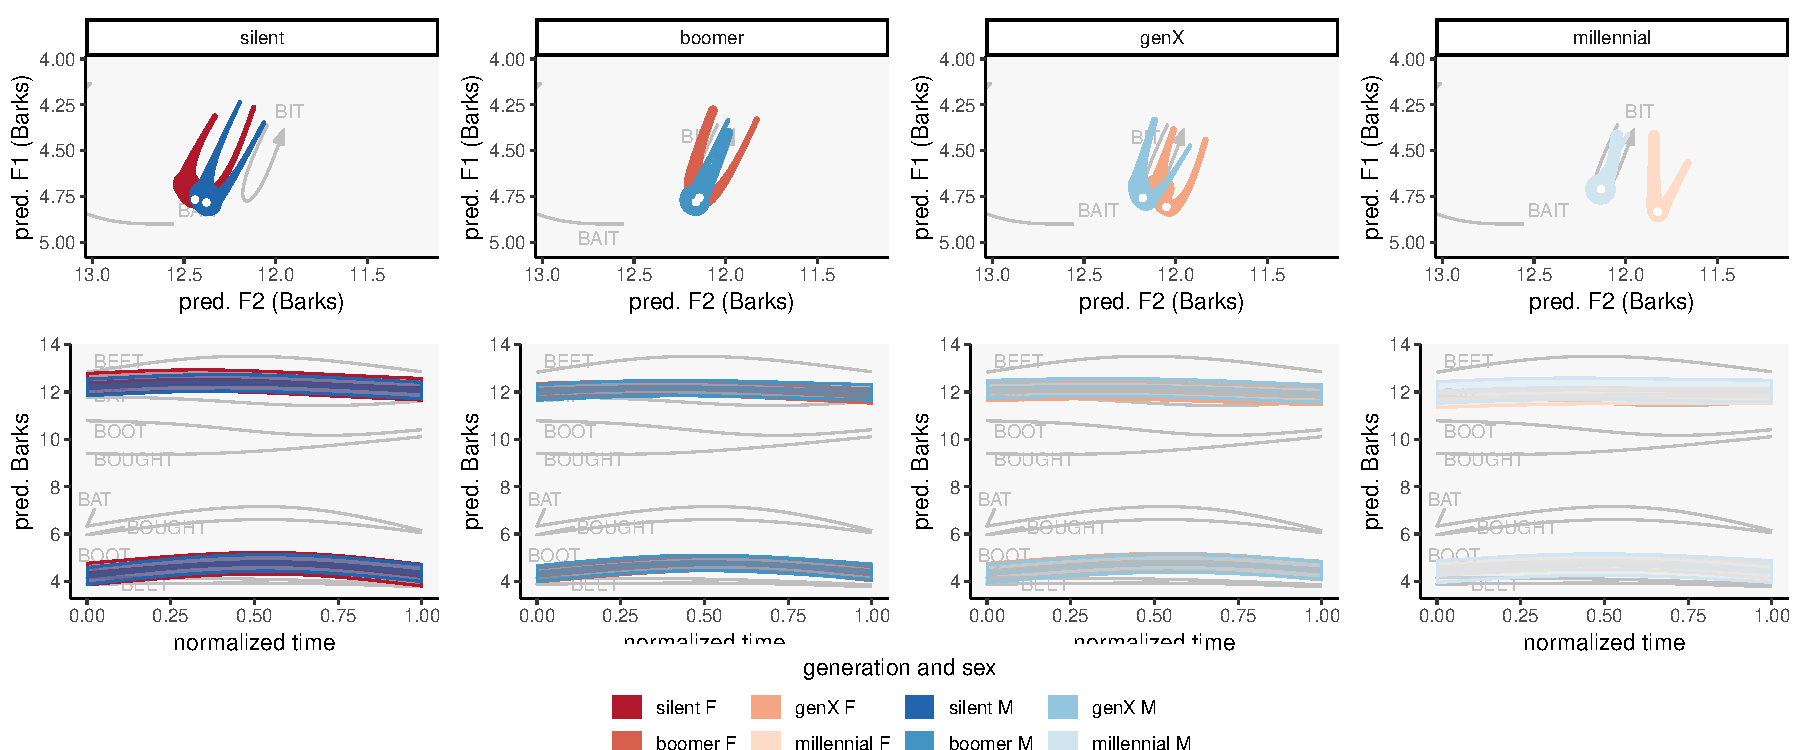
\includegraphics[angle = 90, origin = c, height = \textwidth]{Figures/BIT/BIT_sex_panel_plot_wide.pdf}
	\caption[Predicted formant measurements for \bit by generation.]{Predicted formant measurements for \bit by generation.}
	\label{fig:BIT_sex_panel_plot_wide}
\end{figure*}

A within-generation comparison of men and women, as in Figure \ref{fig:BIT_sex_panel_plot_wide}, illuminates additional insight into how \bit is realized in this community. Basically, there is little difference between the men and women within most generations. Difference smooths suggest that the vowel trajectories of these two sexes were not statistically different in either F1 or F2 (\ref{fig:bit_diff_smooths_sex_gen}A--G). The exception to this are the Millennials, and women's realizations were significantly more retracted than the men's for the first two thirds of the trajectory (\ref{fig:bit_diff_smooths_sex_gen}H). So while the women appear to be shifting more in relation to the men, because the amount of shifting was so small, the differences between the sexes is not apparent until the youngest generation.

Furthermore, there does not appear to be any clear pattern in how the shape of the trajectory changes. There are some changes from a U-shaped pattern to a V-shaped pattern to a ``bounce'' pattern but their distributions appear to be haphazard and generalizations cannot be made. It is possible that because this vowel is so monophthongal that the trajectory itself is not important.

Summarizing the findings for \bit, overall it was the least dynamic vowel and undergoes the smallest amount of change. Women are participating in a pattern of retraction, and \bit is gradually becoming a more centralized vowel, though the amount of change in the vowel space is relatively small. Men retracted somewhat, but for the past three generations the vowel is stable.

\section{Discussion}
\label{sec:preobstruent_discussion}

In the previous sections, I presented the results of generalized additive mixed-effects models on the elsewhere allophones of \trap, \dress, and \kit. This section summarizes these findings, proposes a hybrid of chain shifting and parallel shifting in this community, and links these results with speech patterns found in other communities in the West. I then justify the use of GAMMs by discussing the trajectory-related findings in this chapter.

\subsection{Summary of findings}
\label{bat_bet_bit_summary}

The previous sections have shown that each vowel underwent a variety of changes over time. First, The \bat vowel slowly lowered and retracted in apparent time, with the primary direction of change being in vowel height. In Cowlitz County, this change is being led by the women. In particular the first half of the vowel trajectory shifts more than the last half, meaning that the trajectory shape changes from a V to a bounce. Compared to the other front lax vowels, \bat was the most dynamic.

In women's speech, the \bet vowel lowered and retracted about the same amount while the men's variants of \bet were in approximately the same position in the vowel space. For both sexes, the shape of \bet gradually shifted from a U to a bounce as a result of the first half advancing at a faster rate in apparent time than the second half. The trajectory length of \bet was shorter than \bat, making it a more monophthongal vowel.

\bit undergoes the least amount of change. There was very little change in the vowel height and the retraction found in the women's speech was statistically significant but relatively small. There was no shifting in the men's speech at all. The trajectory shape was inconsistent across generations and devoid of clear patterning. The trajectory length of \bit was a little less than half that of \bat, making it the least dynamic of the front lax vowels.

What do these findings say about the structural relationship of these three vowels in Cowlitz County, and how does this Washington community fit in with neighboring cities?

\subsection{Chain shift, parallel shift, or both?}
\label{sec:what_kind_of_shift}

In \S\ref{sec:structure_of_elsewhere_shift}, I describe how there is inconsistency across regions in how the vowels are shifting. In particular, \citet{boberg_2005} explains that this has implications for whether this movement is a chain shift or a parallel shift. If the vowels undergo a rotation in the vowel space, meaning \bet and \bit lower as \bat retracts and lowers, then there is evidence for a chain shift. However, if the vowels are retracting only, then this may be a parallel shift.

\begin{figure}[tb!]
    \centering
    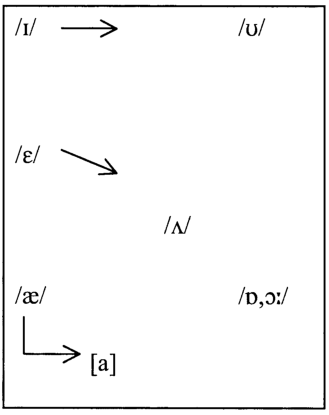
\includegraphics[width = 0.5\textwidth]{Figures/other_figures/montreal_shift.pdf}
    \caption[The Elsewhere Shift in Montreal and Cowlitz County.]{The Elsewhere Shift in Montreal and Cowlitz County. From \citet[149]{boberg_2005}.}
    \label{fig:montreal_shift}
\end{figure}

The patterns found in Cowlitz County are somewhat of a combination of these two idealized scenarios. \bat is lowering with a small amount of retraction, \bet is both lowering and retracting, and \bit is retracting only; all three vowels are moving in different directions. Because \bit is not lowering, a chain shift model---at least one that involves \bit---is not supported. However, because all three vowels do retract to some degree, Cowlitz County vowels very closely match the parallel shift that \citet{boberg_2005} describes in Montreal (Figure \ref{fig:montreal_shift}). However, I cannot ignore the relative timing of when \bet and \bat shift, so the chain shift model seems more appropriate at least for these two lower vowels.
% Donofrio etal 2019 find lowering + retraction in DRESS and TRAP but not KIT. Can I fit that in somewhere?

Perhaps the front lax vowels are not all structurally related; specifically it may be the case that \bet and \bat are chain shifting while \bit is moving independently. Because \bit, \bet, and \bat form a natural class of front lax vowels in English, an elegant description would be that they all move as a unit, but this data suggest that only \bet and \bat are lowering. The \textit{Atlas of North American English} famously includes only \bet lowering and \bat retraction in its definition of the Canadian Shift (in addition to \lot retraction; \citealt[219]{labov_ash_boberg_2006_anae}), so at least in their data \bit was not related to the other two vowels. It may be the case that the Elsewhere Shift in Cowlitz County only applies to the lower two vowels.

An alternative explanation is that the lowering of \bit is the last stage of the chain shift and that these speakers in Cowlitz County have not yet adopted it. Because I cannot predict the future, I cannot use the current dataset to support or reject this hypothesis, but I can use it explore the relative timing of when these vowels shifted.

Beginning with the lowest vowel, Figure \ref{fig:BAT_four_panel} showed that \bat has been shifting for at least four generations.\footnote{This of course assumes the Apparent Time Hypothesis. If speakers adopt elements of the Elsewhere Shift over the course of their lives, the timeline presented here may overestimate the amount of time these shifts have been taking place in the community. Future work will analyze these changes in real time by examining older recordings of speakers in this community.} The difference between the Silent Generation and the Baby Boomers was small, just as it was for every pair of consecutive generations. However, Figure \ref{fig:BAT_sex_panel_plot_wide} showed that women have been leading this change for all the four generations sampled here. The men's realizations approximate those of the women a generation older then them (their mothers). Conservatively then, \bat lowering and retraction began with the women of the Silent Generation and  the oldest men in this sample reflect their mothers' speech (the G.I. Generation) before them.\footnote{It's possible that \bat began shifting began even before the G.I. Generation, but the current dataset cannot offer evidence to support or reject this hypothesis.} In other words, the current sample appears to have captured the lowering and retraction of \bat after it had already began, meaning it started possibly as early as the 1930s. This shifting continued at least through the Millennials, but the difference between the Millennials and Gen X (for either sex) was relatively small. This suggests that perhaps \bat-shifting is nearing completion, though it is likely that Generation Z will continue the shifting to some degree, particularly the men to catch up with the women. So, the data show that \bat had begun shifting at least by 1930s and continued to do so until perhaps the 2000s after the youngest Millennials in this sample were born.

Moving on to \bet, Figure \ref{fig:BET_four_panel} shows that shifting has also occurred in the four generations in this sample. The largest amount of shift for both sexes happened between the oldest generations, or approximately between the 1940s and 1950s. However, Figure \ref{fig:BET_sex_panel_plot_wide} shows that the difference between the sexes in the Silent Generation was negligible. Under the assumption that women lead in language change and that the men lag behind, the fact that the two sexes started off the same suggests no shift had been occurring before the Silent generation. The Baby Boomers were the ones to start lowering and retracting \bet, and they did so quite drastically. There is evidence that the women have stopped shifting because the difference smooths suggest no significant difference between the Gen X and Millennial women. Under this assumption, \bet's movement was completed around the late 1970s and early 1980s. Thus it appears that this sample of Cowlitz County women captures the complete lowering and retraction of \bet: the Baby Boomers started it and the Millennials stopped. It is plausible that the men, who have been relatively stable over the past three generations, will catch up to the women's current lowered and backed position.

Finally, Figure \ref{fig:BIT_four_panel} showed very little lowering of \bit and a somewhat complicated pattern of retraction. Starting with the men this time, \bit retracted between the oldest two generations, but then ceased, suggesting perhaps the final stages of a shift. This was a very similar pattern to \bet. As for the women, \bit retracted between the Silent Generation and the Baby Boomers, remained relatively stable for a generation, and then retracted again with the Millennials. Basically, the pattern is the same as the men, only the Millennials begin retracting again. It is possible then that this sample shows two separate patterns of retraction: the final stages of one that ends with Generation X (for both sexes) and then the start of a new shift (led by the Millennial women).

Taking these three vowels together, the relative timing of these vowels' movement suggests a pull chain in Cowlitz County, with \bat retracting and lowering first and then \bet following suit. \bat has been moving at least since the Silent Generation (perhaps around 1930, if not earlier), and \bet began its movement sometime in the middle of the 20th Century. It is possible then that the Millennial women's sudden retraction of \bit is the next stage of this shift (which started perhaps around the 1980s).

This chain shift hypothesis is strengthened by examining the trajectories of the vowels. For both \bat and \bet, the majority of movement occurred in the first half of the vowel's duration. Figures \ref{fig:BAT_four_panel} and \ref{fig:BET_four_panel} show that the latter portion of the \bat and \bet's trajectories are all approximately the same: it is the first half that shifts towards that offset. Adding \bit into the picture, Figure \ref{fig:BET_four_panel} showed that unlike the other two vowels, the older generations of women retracted the \textit{entire} vowel trajectory. However, after the hiatus between the Baby Boomer and the Generation X women, the Millennial women begin shifting again. Crucially though, this youngest group only differs from Generation X in the first half of \bit's duration---just like the bulk of what happened with \bet and \bat. Therefore, the on-again-off-again \bit retraction that the women show may not be one single pattern but rather is the tail end of one shift and then the Millennial women being early adopters of the Elsewhere Shift. Evidence for this hypothesis from a future sample of Generation Z speakers would show lowering as well retraction in the women's speech, and the start of a shift in the men's.

\subsection{Cowlitz County's place in the West}
\label{sec:cowlitz_place_in_west_preobstruent}

In \S\ref{sec:geography_of_elsewhere_shift}, I synthesize findings from previous studies in the West, showing that the Elsewhere Shift is less clearly defined further north along the Pacific Coast. In California, the lowering of all three vowels is apparent \citep{janoff_2018, hall_lew_etal_2015, cardoso_etal_2016_pads, kennedy_grama_2012, holland_2014_diss}. However, in Oregon, the patterns are a little more haphazard. In the Southern Willamette Valley, younger speakers are lowering \bit, backing \bet, and lowering and backing \bat \citep{nelson_2011}. Just south of Cowlitz County, most Portlanders are retracting \bat \citep{conn_2000_diss, becker_etal_2013}, but fewer lower \bet and a small percentage lower \bit \citep{becker_etal_2016_pads}. North of Cowlitz County, Caucasian Americans in Seattle do not participate in the Elsewhere Shift \citep{wassink_2015, riebold_2015_diss}.

The direction of these individual vowel shifts is different than what was found in Cowlitz County. In this Washington sample, \bat is primarily lowering, \bet is lowering and retracting, and \bit is retracting only. Compared to Oregonians to the South, the directions of change are different, further suggesting that the Elsewhere Shift is less clearly defined north of California. But, at least compared to other Washingtonians to the north, it appears that Cowlitz County speakers are at least adopting aspects of the shift that the Seattleites are not. The amount of shifting may not be as drastic as is found in California, but this data suggests that \bat and \bet have been shifting in Cowlitz County for at least several decades, and perhaps longer. In other words, the Elsewhere Shift, is indeed found in at least one community in Washington.

I tentatively posited above that \bat has been shifting in Cowlitz County since at least the 1930s, that \bet followed suit roughly around 1950s, and then \bit did in the 1980s. How does this timing compare to other regions in the West? In California and Canada, it was found that all three vowels moved at the same time \citep{pratt_etal_2018, donofrio_etal_2019, lawrance_2002_thesis, boberg_2005} so this Washington community does not fit in with those areas. But in Portland, \citet{becker_etal_2016_pads} demonstrate that \bat retracted first, then \bet lowered, and then \bit is just beginning to shift. The relative timing of these changes matches what is found in Cowlitz County. It is unsurprising that Cowlitz County be the most similar to its closest neighbor,\footnote{See \S\ref{sec:portland_vs_seattle} for more on this topic.} but it suggests that the Elsewhere Shift has been present in southwestern Washington at least as long as it has been in Portland and that a \bat-lead chain shift may be more widespread than the Portland area.

Chapter \ref{ch:cowlitz_county}, describes in detail the beginning of Cowlitz County and emphasizes the importance of Long-Bell's establishment in the area. The city of Longview was founded in 1923, and the mills attracted thousands of workers from across the country and the world. This sudden and drastic mixture of dialects in the early 1920s may have been the time that \bat began to lower. \citet{herold_1990_diss} demonstrated that a sudden influx of Eastern European migrant workers triggered the low back merger in mining communities in Eastern Pennsylvania and \citet{johnson_2010_pads} showed how population shifts in New England also triggered that same merger. Thus, sudden demographic changes can be triggers for linguistic change.\footnote{For more on these so-called \textit{catastrophic events}, see \citet{bailey_etal_1996}, \citet{bailey_2018}, \citet{schilling_2017}, \citet{carmichael_2017}, and \citet[24]{labov_1994}.} If the Elsewhere Shift is the result of purely structural and language-internal pressures, then it is conceivable that the shift developed independently in Cowlitz County---especially since it was not until 1925 that Washingtonians were the majority population in Cowlitz County.

On the other hand, \S\ref{sec:longview_a_planned_city} explains that despite a large proportion of 1930 Cowlitz County being from outside Washington, the majority of non-Washingtonian Americans came from Oregon and the majority of foreign-born immigrants were from Canada. If the beginning of the Elsewhere Shift was already established in those areas (namely the retraction and lowering of \bat), those immigrants may have simply brought the speech patterns into the area. The Founder Principle \citep{zelinsky_1973, mufwene_1996} predicts that this not be possible and that the original English-speaking settlers to the area\footnote{We actually know the first three English-speaking settlers of Cowlitz County: Englishman Adophus Le Lewes, Qu{\'e}b{\'e}cois Simon Plamondon, and Scotsman Peter Crawford. See \S\ref{sec:exploration_discovery} and \ref{sec:settlement_colonization}.} have the most influence. However, language continues to change and there are cases where original founder dialect features are erased as majority language patterns take over \citep{stanford_etal_2012}. Perhaps the sudden influx of immigrants from many dialect areas---chief among them Canada and Oregon---helped begin the lowering of \trap.

With the current sample of Cowlitz County speakers, I am unable to confirm whether the Elsewhere Shift was an internal development or imported from other communities. However, the timing of \bat retraction coincides with the founding of Longview, suggesting that the subsequent demographic shift at least play a part. Additional research, particularly on recordings of people born before 1923, may shed some needed light on this topic.





\subsection{Trajectories and the Elsewhere Shift}
\label{sec:trajs_and_elsewhere_shift}

The previous section emphasized the relative position of the vowels in the vowel space while paying attention to their trajectories. To my knowledge, this is the first detailed account of the trajectory of all three front lax vowels in relation to the Elsewhere Shift. What does this additional complexity mean and was the use of GAMMs warranted?

I argue that analyzing the full trajectories of these vowels enhances what is known about the Elsewhere Shift. \bat and \bet primarily shifted during the first halves of their trajectories, and because the same pattern is found in the Millennial women, it is possible that \bit is following suit. Therefore, in Cowlitz County, it appears that the Elsewhere Shift is \textit{not} simply a change in vowel nuclei but that the entire first half of the trajectory is what shifts. And because the second half undergoes relatively less movement, the result is a change in the shape as well: the vowels go from a U-shape to a ``bounce.''

\begin{figure*}[tb!]
    \centering
    \hspace{\fill}
    \begin{subfigure}[t]{2.925in} % 0.45\textwidth
        \centering
        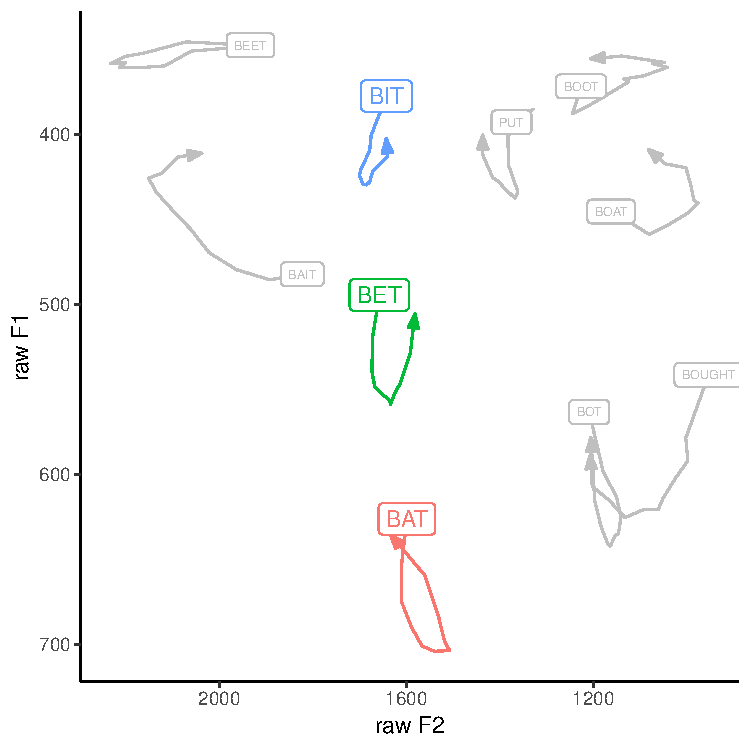
\includegraphics[width = \textwidth]{Figures/example_plots/51-Rich_avg_traj.pdf}
        \caption{Rich's trajectories are more U-shaped.}
        \label{fig:avg_traj_rich}
    \end{subfigure}
    \hspace{\fill}
    \begin{subfigure}[t]{2.925in}
        \centering
        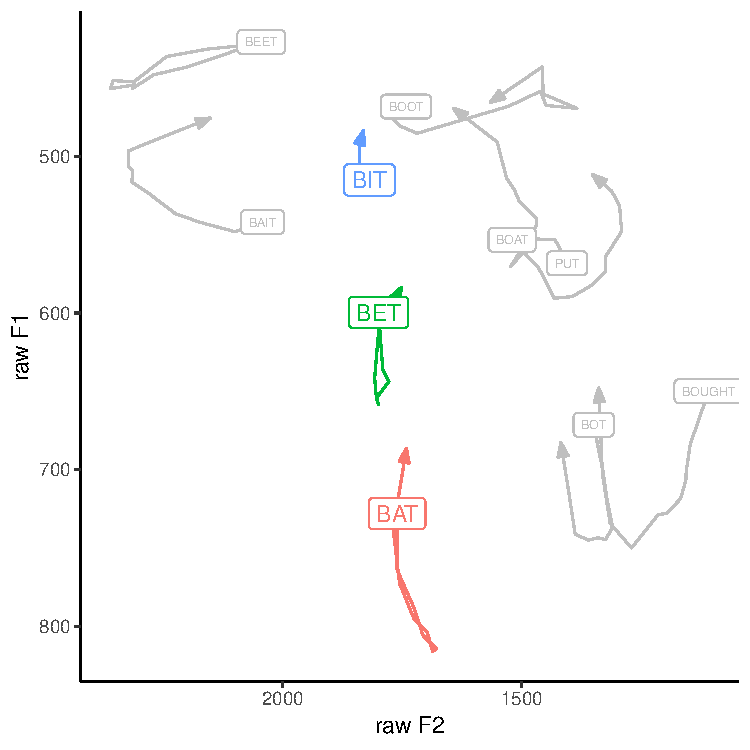
\includegraphics[width = \textwidth]{Figures/example_plots/54-Amber_avg_traj.pdf}
        \caption{Amber's trajectories are more ``bounce''-shaped.}
        \label{fig:avg_traj_amber}
    \end{subfigure}
    \hspace{\fill}
    \caption{Average trajectories (in unnormalized Hz) for two Cowlitz County speakers showing the beginning and end stages of the Elsewhere Shift.}
    \label{fig:rich_and_amber}
\end{figure*}

The predicted values from the GAMMs however, are idealized trajectories. Does this claim hold up when the raw data is examined? Figure \ref{fig:avg_traj_rich} shows the average trajectories for Rich, a male Baby Boomer born in 1957. The trajectories of Rich's front lax vowels exhibit the characteristic U-shape found in the older generations. In other words, while F1 gradually raises and then lowers, F2 undergoes a small amount of lowering. Meanwhile, Figure \ref{fig:avg_traj_amber} is of Amber, a female Millennial born in 1995. Here, we see a clear ``bounce'' pattern that these models predict in the younger speakers: the F2 of these three vowels hardly changes at all and the trajectory changes in vowel height only.\footnote{It is difficult to compare the relative position of these speakers' vowels because the data is unnormalized. The only points of reference are the speakers' other vowels, but those too are in flux. However, compared to \fleece and \face, it appears that the lax vowels are lower in Amber's speech than in Rich's, supporting the chain shift as well.} These two speakers exemplify the change in trajectory shape and support the idea that the Elsewhere Shift is more than a change in position but is also  change in vowel trajectory.

\begin{figure*}[tb!]
    \centering
    \hspace{\fill}
    \begin{subfigure}[t]{2.925in}
        \centering
        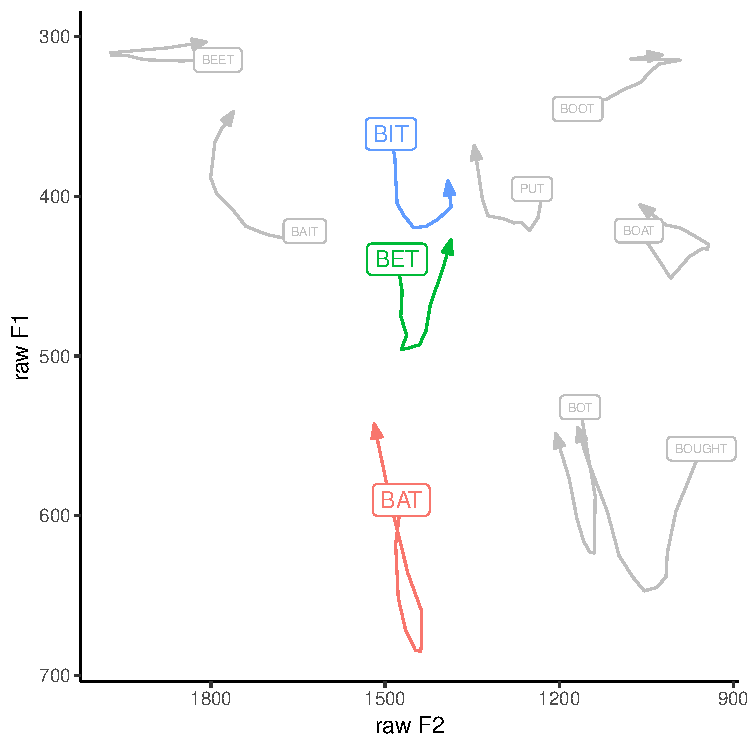
\includegraphics[width = \textwidth]{Figures/example_plots/30-Jason_avg_traj.pdf}
        \caption{Jason's \bat is ``bounced'' while \bet and \bit are U-shaped.}
        \label{fig:avg_traj_jason}
    \end{subfigure}
    \hspace{\fill}
    \begin{subfigure}[t]{2.925in}
        \centering
        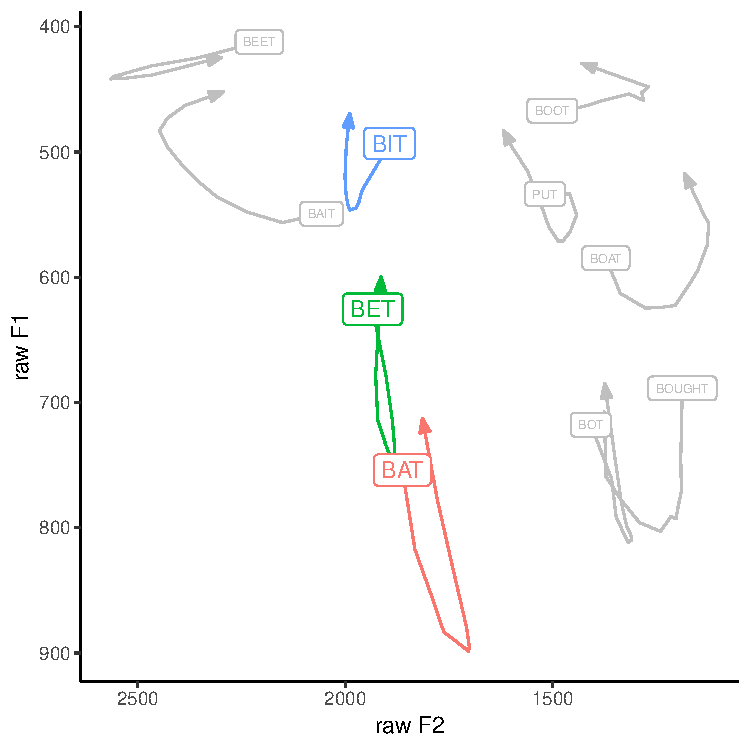
\includegraphics[width = \textwidth]{Figures/example_plots/29-Amanda_avg_traj.pdf}
        \caption{Amanda's \bat and \bet are ``bounced'' while \bit is U-shaped.}
        \label{fig:avg_traj_amanda}
    \end{subfigure}
    \hspace{\fill}
    \caption{Average trajectories (in unnormalized Hz) for two Cowlitz County speakers showing intermediate stages of the Elsewhere Shift.}
    \label{fig:jason_and_amanda}
\end{figure*}

The intermediate steps of this chain shift can also be found in these raw data plots. Figure \ref{fig:avg_traj_jason} shows the average trajectories for Jason, a male from male from Generation X born in 1974. Jason's vowels show the first stages of the Elsewhere Shift with a ``bounce''-like pattern for \bat but not for \bet or \bit. Jason is one generation younger than Rich (Figure \ref{fig:avg_traj_rich}) which supports the relative timing of the shift. Meanwhile, Figure \ref{fig:avg_traj_amanda} shows the vowels of Amanda, a female Millennial born in 1990. Here, both \bat and \bet have relatively little change in F2, while \bit is still U-shaped. Amanda appears to be a late adopter within her generation since \bit does not yet pattern with the other two vowels. These two speakers exemplify the intermediate stages of the Elsewhere Shift and show the relative timing of each vowel's changes.

\begin{figure*}[tb!]
    \centering
    \hspace{\fill}
    \begin{subfigure}[t]{2.925in}
        \centering
        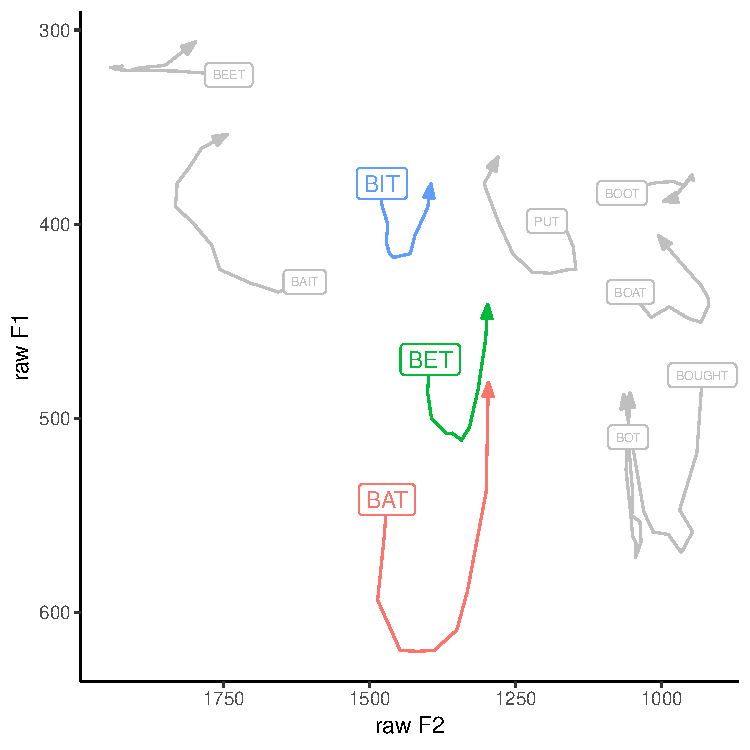
\includegraphics[width = \textwidth]{Figures/example_plots/35-Craig_avg_traj.pdf}
        \caption{Craig is a late adopter with his U-shaped trajectories.}
        \label{fig:avg_traj_craig}
    \end{subfigure}
    \hspace{\fill}
    \begin{subfigure}[t]{2.925in}
        \centering
        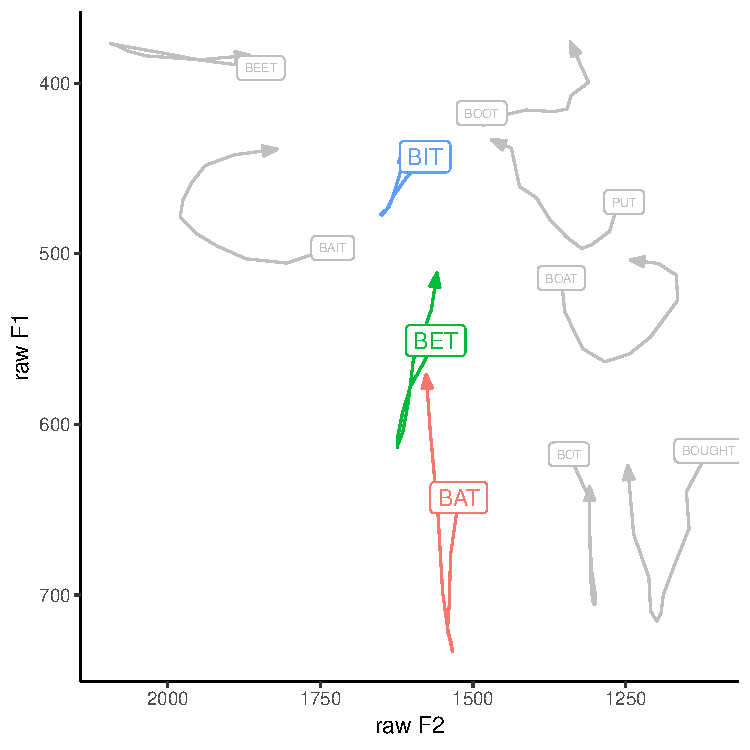
\includegraphics[width = \textwidth]{Figures/example_plots/47-Sean_avg_traj.pdf}
        \caption{Sean is an early adopter with his ``bounce''-like trajectories.}
        \label{fig:avg_traj_sean}
    \end{subfigure}
    \hspace{\fill}
    \caption{Average trajectories (in unnormalized Hz) for two Cowlitz County speakers.}
    \label{fig:craig_and_sean}
\end{figure*}

Two additional plots shed some light as to the social meaning of the Elsewhere Shift in Cowlitz County. Figure \ref{fig:avg_traj_craig} shows the average trajectories of Craig, a male Baby Boomer born in 1962. Despite other men his age adopting some of the shift (like Rich above), Craig appears to lag behind and exhibits clear U-shaped trajectories for all three front lax vowels. Meanwhile Figure \ref{fig:avg_traj_sean} shows Sean, a male Millennial born in 1985. He is on the older end of his generation, but still has elements of the shift in all three vowels. Craig grew up in the rural north side of Cowlitz County, spoke fondly of the Longview's ``good ol' days,'' and rarely goes to Portland. Meanwhile, Sean grew up in the heart of Longview, expressed disdain towards Longview, and goes to Portland frequently to attend (or play in) concerts.\footnote{In chapter \ref{ch:discussion} we will hear more from both Craig and Sean and how they exemplify general community views towards Longview and Portland.} The correlation between their speech patterns and their views towards local places sheds some light on the social meaning of the Elsewhere Shift in Cowlitz County. This topic will be treated in more detail in Chapter \ref{ch:discussion}.

Finally, I want to again point out the pattern found for \bet. While women were shifting the relative position of the vowel to a lower and more retracted position, both sexes were changing its shape from a U-shape to a bounce. Language change in Western cultures has shown that women are in the lead and that the men lag behind by a generation or so (as I have shown in this chapter). However, it may be that some aspects of the shift, namely the trajectories, advance equally in all social groups. While the men are not lowering or retracting \bet as the women are, the two sexes are in-step as they change the trajectory from more U-shaped to a ``bounce.'' Additional work on trajectories in sound change are needed to see if this is a pattern found elsewhere, but it begs the question of how much information is missed when single-point measurements are used and trajectories are ignored.



\section{Conclusion}
\label{bat_bet_bit_conclusion}

This chapter has taken a close look at \bat, \bet, and \bit in Cowlitz County, Washington, giving particular emphasis on their trajectories. The front lax vowels are shifting in Cowlitz County, but the nature of the shift suggests a combination of a parallel shift and a pull chain. The relative timing of vowel lowering clearly indicates that \bat began shifting before \bet did, and that both vowels' movements are nearing completion. For \bit, there is evidence in the trajectory that it is beginning to shift as well in the Millennial women's speech. For all three vowels, the first half is shifting faster than the second half, causing a change in the trajectory shape from a U-shape to a curve. In other words, there is less and less movement in F2 in these vowels in apparent time. These patterns are supported by examining data from individual speakers. In conclusion, the Elsewhere Shift can be found in Cowlitz County, Washington and it involves a change in trajectory as well as a change in position.
